\section{Game Design}

The goal for this game was to have two players communicate and collaborate with each other in order to push a block to a certain location on the screen, the goal. The game consists of two different screens of the same size: one that is only visible to player one and another that is only visible to player two. Figure one shows an example screen for player one and two. 
\\*

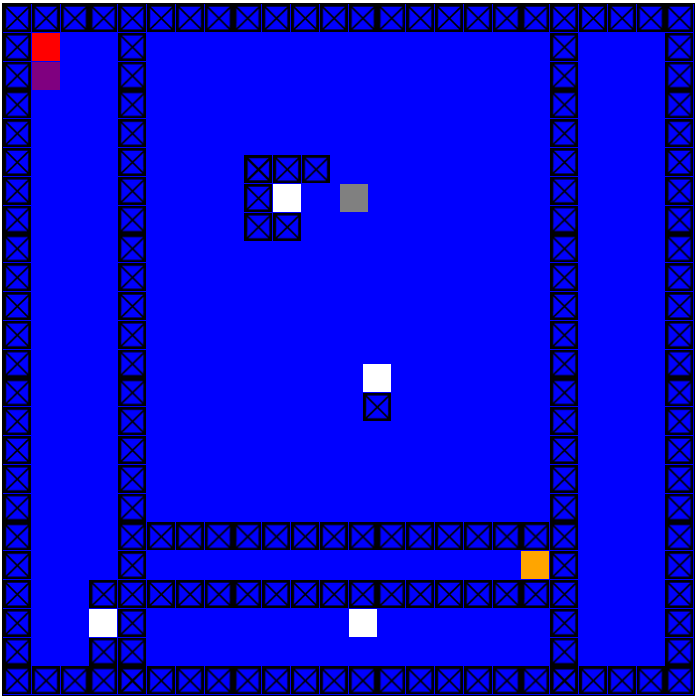
\includegraphics[scale=0.27]{playerview1.png} 
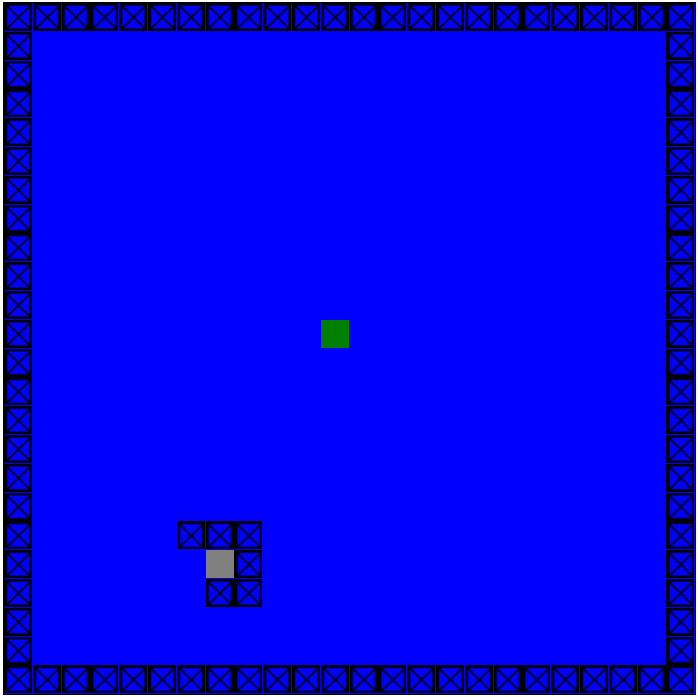
\includegraphics[scale=0.27]{playerview2.png}
 	 
Figure 1: This shows an example of the differences between the screens of player one and player two. The screenshot on the right is the screen player one sees on level two. The red square is the player character and the orange square is the goal block. The purple block is the block that needs to be pushed to the goal. On the left is player two’s screen. The green square is the player character.
\\*
\\*
On each screen is a maze created from various obstacles that must be overcome in order to push the block to the goal block. The obstacles can be overcome by the strategic placement of blocks that each player can place on their partner's screen. However, since each players' screen is invisible to their partner, players must provide typed instructions leading to the precise location that a block needs to be placed. Players must interpret the directions and move to the position they believe that their partner is describing. Players can then place a block on their partner's screen at the same position that they currently are on their own screen. Each player can only place three blocks on their partner's screen at a time. After three blocks are placed on their partner's screen, when another block is placed, the block that was placed the first is deleted to make room for the new block. Figure 2 shows an example of this.
\\*

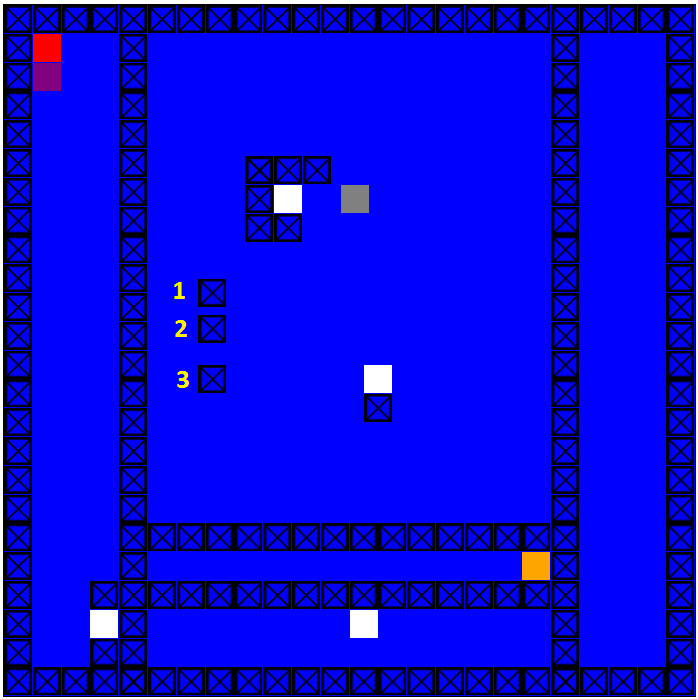
\includegraphics[scale=0.27]{blocksplaced1.png}
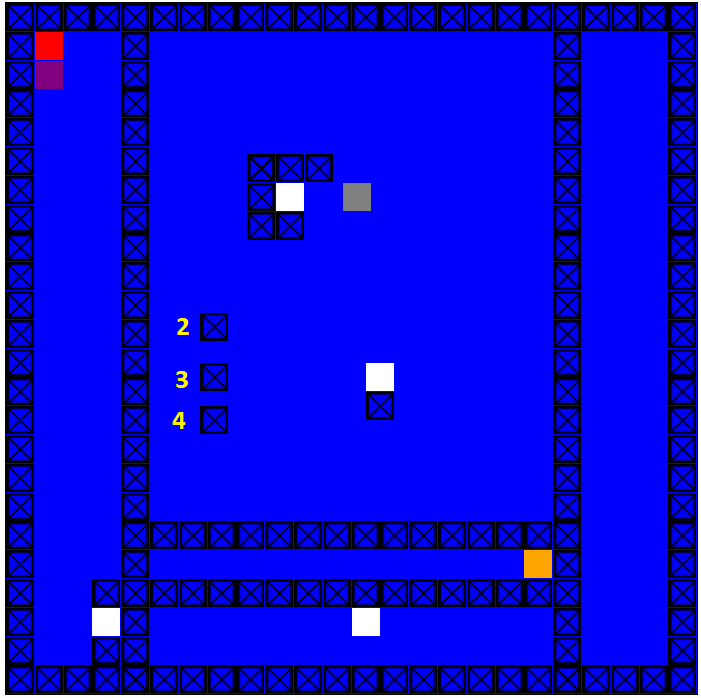
\includegraphics[scale=0.27]{blocksplaced2.png}

Figure 2: This figure illustrates what happens when more than three blocks are placed by player two. The picture on the left shows a screenshot with three blocks already placed in a line in the near the middle of the screen. The numbers next to the blocks correspond to when they were placed. For example, the block with the one next to it was the first block placed and so on. The picture on the right shows what happens when another block is placed after three are already placed. The block that gets deleted was the first of all the blocks placed in the left picture.
\\*
\\*
To further increase the difficulty, the block that the players must push into the goal can only move in one direction at a time. Once a player pushes the ball in a certain direction by moving their character into it, the block will continue moving in that direction and will not stop until it collides with an obstacle. The only thing that can stop the player when they are moving is if they run into a wall or a block dropped by player two. The mazes are designed so that this restriction prevents a player from pushing the block into the goal without any help from their partner. This forces the players to work together since they cannot succeed without one another.